\documentclass[12pt]{article}
\usepackage[polish]{babel}
\usepackage{float}
\usepackage{listings}
\usepackage[utf8]{inputenc}
\usepackage{amsmath}
\usepackage{pdfpages}
\usepackage[T1]{fontenc} % Add this line
    \title{Sprawozdanie z projektu MOM}
    \author{Krzysztof Rudnicki, 307585}
    \date{\today}
\begin{document}

\maketitle
\section{Zadanie 1. Sieć przepływowa}

\subsection{Model sieciowy}
\paragraph{Problem do rozwiązania}
Należy rozwiązać problem najtańszego przepływu \\
\begin{figure}[htb]
\caption{Koszty transportowe i przepustowości na poszczególnych odcinkach}
\begin{center}
\begin{tabular}{ | c | c | c | c | c | c | }
\hline
  & D & E & F & G & H \\ 
 \hline
 A & 4, 15 & 2, 10 & - & - & -\\  
 \hline
 B & 4, 4 & 3, 9 & - & 8, 9 & - \\
 \hline  
 C & 2, 20 & 6, 10 & - & - & - \\
 \hline  
 D & - & - & 3, 10 & 7, 3 & 2, 2 \\
 \hline  
 E & 5, 20 & - & 7, 5 & 6, 5 & 3, 5 \\
 \hline  
\end{tabular}
\end{center}
\end{figure}
\begin{figure}[htb]
\caption{Zdolności wydobywcze kopalń (w tys. ton)}
\begin{center}
\begin{tabular}{ | c | c |}
\hline
  $W_A$ & 10 \\
 \hline
$W_B$ & 13 \\
 \hline
 $W_C$ & 17 \\
 \hline  
\end{tabular}
\end{center}
\end{figure}
\begin{figure}[htb]
\caption{Średnie zużycie dobowe węgla przez elektronie (w tys. ton)}
\begin{center}
\begin{tabular}{ | c | c |}
\hline
  $Z_F$ & 15 \\
 \hline
$Z_G$ & 13 \\
 \hline
 $Z_H$ & 7 \\
 \hline  
\end{tabular}
\end{center}
\end{figure}
\paragraph{Sformułowanie}
Matematyczne sformułowanie zadania:
\begin{enumerate}
\item Parametry \\
s - źródło \\
B - Budynki (kopalnie, stacje, elektrownie) \\
K - kopalnie \\
$c_{ij}$ - koszt transportu z budynku i do budynku j ($c_{sk}$ = 0) \\ 
$W_k$ - zdolność wydobywcza kopalni k [w tonach] \\ 
$p_{ij}$ - przepustowość transportu z budynku i do budynku j [w tonach] ($u_{sk}$ = $W_k$) \\ 
E - elektrownie \\ 
$Z_e$ - średnie zużycie dobowe przez elektrownię e [w tonach] \\  
\item Zmienne decyzyjne
$f_{ij}$ - przepływ transportu z budynku i do obiektu j \\ 
\item Funkcja celu
\begin{align*}
    Q &= \min\left(\sum_{(i, j) \in B \backslash \{s\}} c_{ij} f_{ij}\right) \\
    &= \min(4f_{AD} + 2f_{AE} + 4f_{BD} + 3f_{BE} + 8f_{BG} + 2f_{CD} \\
    &\quad + 6f_{CE} + 3f_{DF} + 7f_{DG} + 2f_{DH} + 5f_{ED} + 7f_{EF} \\
    &\quad + 6f_{EG} + 3f_{EH})
\end{align*}

\item Ograniczenia
\begin{equation}
    0 \leq f_{sk} \leq W_k, \; k \in K = \{A, B, C\}
\end{equation}
\begin{equation}
    f_{si} = 0, \; i \in B \backslash K
\end{equation}
\begin{equation}
    f_{is} = 0, \; i \in B
\end{equation}
\begin{equation}
    0 \leq f_{ij} \leq p_{uj}, \; (i, j) \in B \backslash \{s\}
\end{equation}
\begin{equation}
    f_{is} = 0, \; i \in B
\end{equation}
\begin{equation}
    \sum_{b \in B} f_{be} \ge Z_e, \; e \in E = \{F, G, H\}
\end{equation}
\begin{equation}
    \sum_{i \in B \backslash \{ s \} } f_{bi} \leq \sum_{j \in B} f_{bn}, \; b \in B \backslash \{s\}
\end{equation}

\end{enumerate}
\paragraph{Narysowanie modelu}
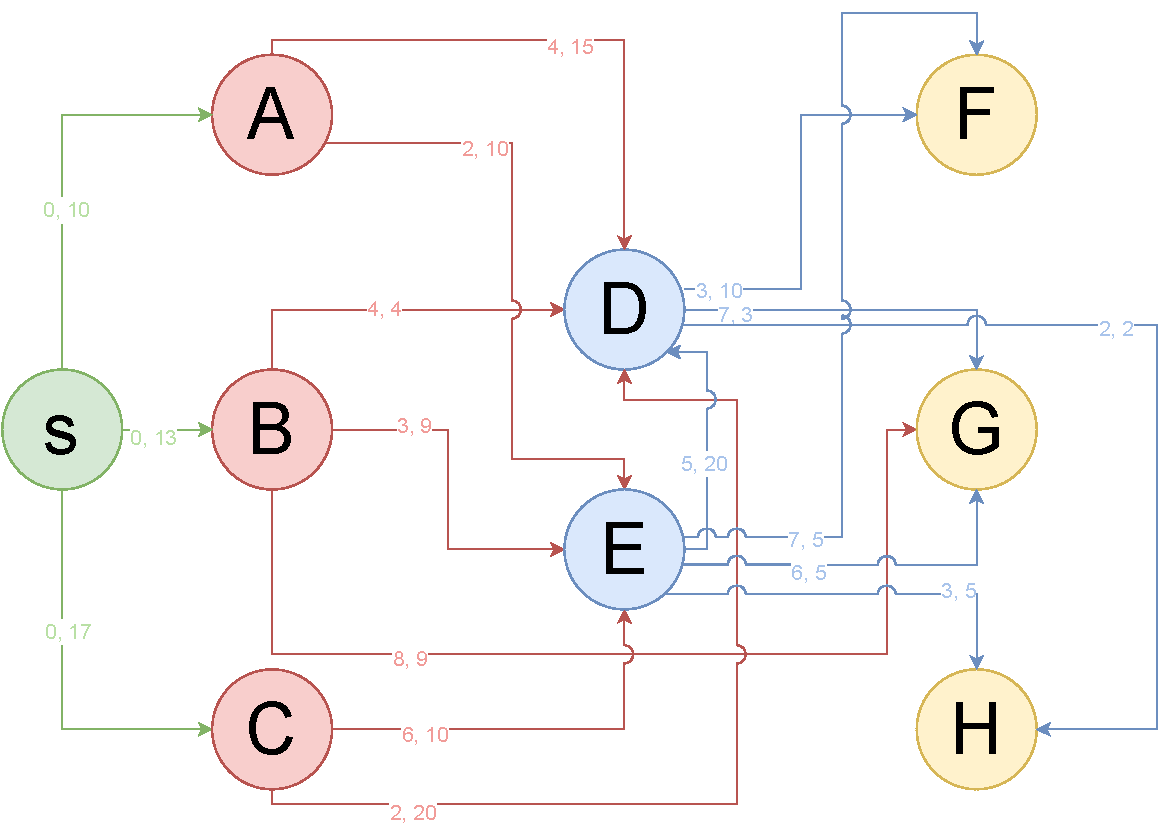
\includepdf[pages=-]{1flow.pdf}

\subsection{Rozwiązanie}
\paragraph{Zadanie programowania liniowego}

\begin{lstlisting}[caption= plik dat]
data; 
 
set BudynkiNaStart := s, A, B, C, D, E, F, G, H; 
set Budynki := A, B, C, D, E, F, G, H; 
set Elektrownie := F, G, H; 

param Z := F 15 G 13 H 7; 
 
param p := 
s A 10 s B 13 s C 17 s D 0  s E 0  s F 0  s G 0  s H 0
A A 0  A B 0  A C 0 A D 15  A E 10 A F 0  A G 0  A H 0
B A 0  B B 0  B C 0 B D 4 B E 9  B F 0  B G 9  B H 0
C A 0  C B 0 C C 0 C D 20 C E 10 C F 0  C G 0  C H 0   
D A 0  D B 0  D C 0  D D 0 D E 0 D F 10 D G 3   D H 2 
E A 0  E B 0  E C 0 E D 20 E E 0 E F 5 E G 5  E H 5  
F A 0  F B 0  F C 0  F D 0  F E 0  F F 0  F G 0  F H 0
G A 0  G B 0  G C 0 G D 0  G E 0  G F 0  G G 0  G H 0
H A 0  H B 0  H C 0  H D 0  H E 0  H F 0  H G 0 H H 0; 
 
param c := 
s A 0 s B 0 s C 0 s D 0 s E 0 s F 0 s G 0 s H 0
A A 0 A B 0 A C 0 A D 4  A E 2 A F 0 A G 0 A H 0
B A 0 B B 0 B C 0 B D 4 B E 3 B F 0 B G 8 B H 0
C A 0 C B 0 C C 0 C D 2 C E 6 C F 0 C G 0 C H 0   
D A 0 D B 0 D C 0 D D 0 D E 0 D F 3 D G 7 D H 2
E A 0 E B 0 E C 0 E D 5  E E 0 E F 7 E G 6 E H 3 
F A 0 F B 0 F C 0 F D 0 F E 0 F F 0 F G 0 F H 0
G A 0 G B 0 G C 0 G D 0 G E 0 G F 0 G G 0 G H 0
H A 0 H B 0 H C 0 H D 0 H E 0 H F 0 H G 0 H H 0; 

end; 
\end{lstlisting}
\begin{lstlisting}[caption= plik mod]
set BudynkiNaStart; 
set Budynki; 
set Elektrownie; 

param Z{e in Elektrownie}; 
param p{i in BudynkiNaStart, j in Budynki}; 
param c{i in BudynkiNaStart, j in Budynki}; 

var f{i in BudynkiNaStart, j in Budynki}, >= 0; 
 
minimize Q: sum {i in Budynki, j in Budynki} c[i,j] * f[i,j]; 
 
subject to 
  Ograniczenie_jeden{i in BudynkiNaStart, j in Budynki}: 
    f[i,j] >= 0; 
  Ograniczenie_dwa{i in BudynkiNaStart, j in Budynki}: 
    f[i,j] <= p[i,j]; 
  Ograniczenie_trzy{e in Elektrownie}: 
      sum {n in BudynkiNaStart} f[n,e] >= Z[e]; 
  Ograniczenie_cztery{n in Budynki}: 
    sum {i in Budynki} f[n,i] <= sum {j in BudynkiNaStart} f[j,n]; 
 
solve; 
display {i in Budynki, j in Budynki: f[i,j] > 0}: f[i,j]; 
display: Q;
\end{lstlisting}
\paragraph{Wynik}
\begin{lstlisting}[caption=Wynik z glpk]
f[A,E].val = 10
f[B,E].val = 4
f[B,G].val = 9
f[C,D].val = 12
f[D,F].val = 10
f[D,H].val = 2
f[E,F].val = 5
f[E,G].val = 4
f[E,H].val = 5
Q.val = 236
\end{lstlisting}

\begin{figure}[htb]
\caption{Plan dostaw węgla}
\begin{center}
\begin{tabular}{ | c | c | c | c | c | c | }
\hline
  & D & E & F & G & H \\ 
 \hline
 A & 10 & - & - & - & -\\  
 \hline
 B & 0 & 4 & - & 9 & - \\
 \hline  
 C & 12 & - & - & - & - \\
 \hline  
 D & - & - & 10 & - & 2 \\
 \hline  
 E & - & - & 5 & 4 & 5 \\
 \hline  
\end{tabular}
\end{center}
\end{figure}

\[ Q = 236 \]

\subsection{Wąskie gardło}
Następny szukamy przekroju o jak najmniejszej przepustowości \\
W tym celu usunęliśmy parametry dotyczące średniego zużycia dobowego oraz kosztów transportu i zostawiliśmy wyłącznie przepustowość
\begin{lstlisting}[caption= plik dat]
data; 
 
set BudynkiNaStart := s, A, B, C, D, E, F, G, H; 
set Budynki := A, B, C, D, E, F, G, H; 
set Elektrownie := F, G, H; 
 
param p := 
s A 10 s B 13 s C 17 s D 0  s E 0  s F 0  s G 0  s H 0
A A 0  A B 0  A C 0 A D 15  A E 10 A F 0  A G 0  A H 0
B A 0  B B 0  B C 0 B D 4 B E 9  B F 0  B G 9  B H 0
C A 0  C B 0 C C 0 C D 20 C E 10 C F 0  C G 0  C H 0   
D A 0  D B 0  D C 0  D D 0 D E 0 D F 10 D G 3   D H 2 
E A 0  E B 0  E C 0 E D 20 E E 0 E F 5 E G 5  E H 5  
F A 0  F B 0  F C 0  F D 0  F E 0  F F 0  F G 0  F H 0
G A 0  G B 0  G C 0 G D 0  G E 0  G F 0  G G 0  G H 0
H A 0  H B 0  H C 0  H D 0  H E 0  H F 0  H G 0 H H 0; 
 
end; 
\end{lstlisting}
\begin{lstlisting}[caption= plik mod]
set BudynkiNaStart; 
set Budynki; 
set Elektrownie; 
 
param p{i in BudynkiNaStart, j in Budynki}; 
 
var f{i in BudynkiNaStart, j in Budynki}, >= 0; 
 
maximize Q: sum {i in Budynki, e in Elektrownie} f[i,e]; 
 
subject to 
  Ograniczenie_jeden{i in BudynkiNaStart, j in Budynki}: 
    f[i,j] >= 0; 
  Ograniczenie_dwa{i in BudynkiNaStart, j in Budynki}: 
    f[i,j] <= p[i,j]; 
  Ograniczenie_trzy{n in Budynki}: 
    sum {i in Budynki} f[n,i] <= sum {j in BudynkiNaStart} f[j,n]; 
 
solve; 
display {i in Budynki, j in Budynki: f[i,j] > 0}: f[i,j]; 
display: Q;
\end{lstlisting}

\paragraph{Wyniki}
\begin{lstlisting}[caption=Wynik z glpk]
f[A,D].val = 9
f[A,E].val = 1
f[B,E].val = 4
f[B,G].val = 9
f[C,D].val = 6
f[C,E].val = 10
f[D,F].val = 10
f[D,G].val = 3
f[D,H].val = 2
f[E,F].val = 5
f[E,G].val = 5
f[E,H].val = 5
Q.val = 39
\end{lstlisting}

\begin{figure}[htb]
\caption{Wyniki poszukiwań wąskiego gardła}
\begin{center}
\begin{tabular}{ | c | c | c | c | c | c | }
\hline
  & D & E & F & G & H \\ 
 \hline
 A & 9 & 1 & - & - & -\\  
 \hline
 B & - & 4 & - & 9 & - \\
 \hline  
 C & 6 & 10 & - & - & - \\
 \hline  
 D & - & - & 10 & 3 & 2 \\
 \hline  
 E & - & - & 5 & 5 & 5 \\
 \hline  
\end{tabular}
\end{center}
\end{figure}

\[ Q = 39 \]

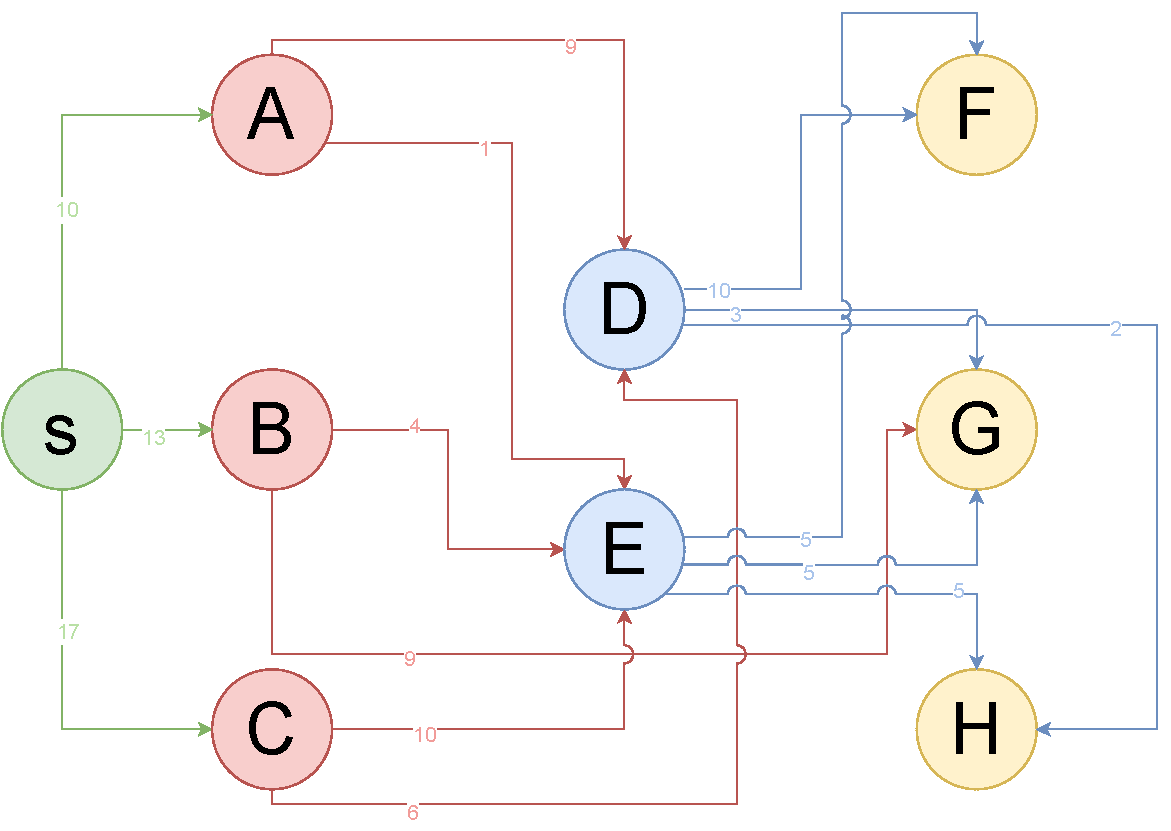
\includepdf[pages=-]{flow12.pdf}

\paragraph{Wnioski}
Następujące przepływy są zbyt niskie w porównaniu do przepustowości:
\[ p_{AD} = 9 \le 15  \]
\[ p_{AE} = 1 \le 10  \]
\[ p_{BE} = 4 \le 9  \]
\[ p_{CD} = 6 \le 20  \]
Zwiększenie przepływów do poziomu maksymalnej przepustowości zwiększyło by wydajność sieci



\section{Zadanie 2. Zadanie przydziału}
\subsection{Zadanie 2.1 Planowanie realizacji portfela przy ograniczonych kompetencjach}
\begin{figure}[htb]
\caption{Kompetencje zespołów}
\begin{center}
\begin{tabular}{ | c | c | c | c | c | c | c | }
\hline
  & A & B & C & D & E & F \\ 
 \hline
 1 & - & X & - & X & X & - \\  
 \hline
 2 & - & X & X & - & X & - \\
 \hline  
 3 & X & - & - & X & - & X \\
 \hline  
 4 & X & - & X & - & - & X \\
 \hline  
 5 & - & X & - & - & X & X \\
 \hline  
 6 & X & - & X & X & - & - \\
 \hline
\end{tabular}
\end{center}
\end{figure}
\subsubsection{Problem do rozwiązania}
\paragraph{Sformułowanie}
Matematyczne sformułowanie zadania:
\begin{enumerate}
\item Parametry \\
s - źródło \\
w - wyjście \\
N - węzły (N = {s, t, 1, 2, 3, 4, 5, 6, A, B, C, D, E, F})
P - projekty (P = {1, 2, 3, 4, 5, 6} $\subseteq$ N)
Z - zespoły (Z = {A, B, C, D, E, F} $\subseteq$ N)
$u_{ij}$ - przepustowość pomiędzy węzłem i a węzłem j
\item Zmienne decyzyjne
$f_{ij}$ - przepływ między węzłem i a węzłem j
\item Funkcja celu
\begin{align*}
    Q &= \max\left(\sum_{p \in P} f_{pt} \right) \\
    &= \max(f_{1t} + f_{2t} + f_{3t} + f_{4t} + f{5t} + f_{6t})
\end{align*}

\item Ograniczenia
\setcounter{equation}{0}
\begin{equation}
0 \leq f_{ij} \leq 1, (i, j) \in N
\end{equation}
\begin{equation}
0 \leq f_{zp} \leq u_{zp}, z \in Z, p \in P
\end{equation}
\begin{equation}
f_{si} = 0, i \in \{ s, t, 1, 2, 3, 4, 5, 6 \}
\end{equation}
\begin{equation}
f_{is} = 0, i \in N
\end{equation}
\begin{equation}
f_{ti} = 0, i \in N
\end{equation}
\begin{equation}
f_{it} = 0, i \in \{s, t, A, B, C, D, E, F\}
\end{equation}
\begin{equation}
\sum_{z \in Z} f_{zp} = 1, p \in P = \{ 1, 2, 3, 4, 5, 6 \}
\end{equation}

\begin{equation}
\sum_{p \in P} f_{zp} = 1, z \in Z = \{ A, B, C, D, E, F \}
\end{equation}

\begin{equation}
\sum_{i \in N \backslash \{s\}} f_{ni} = \sum_{j \in N \backslash \{t\}} f_{jn}, n \in N \backslash \{ s, t \}
\end{equation}



\end{enumerate}

\paragraph{Model sieciowy rysunek}
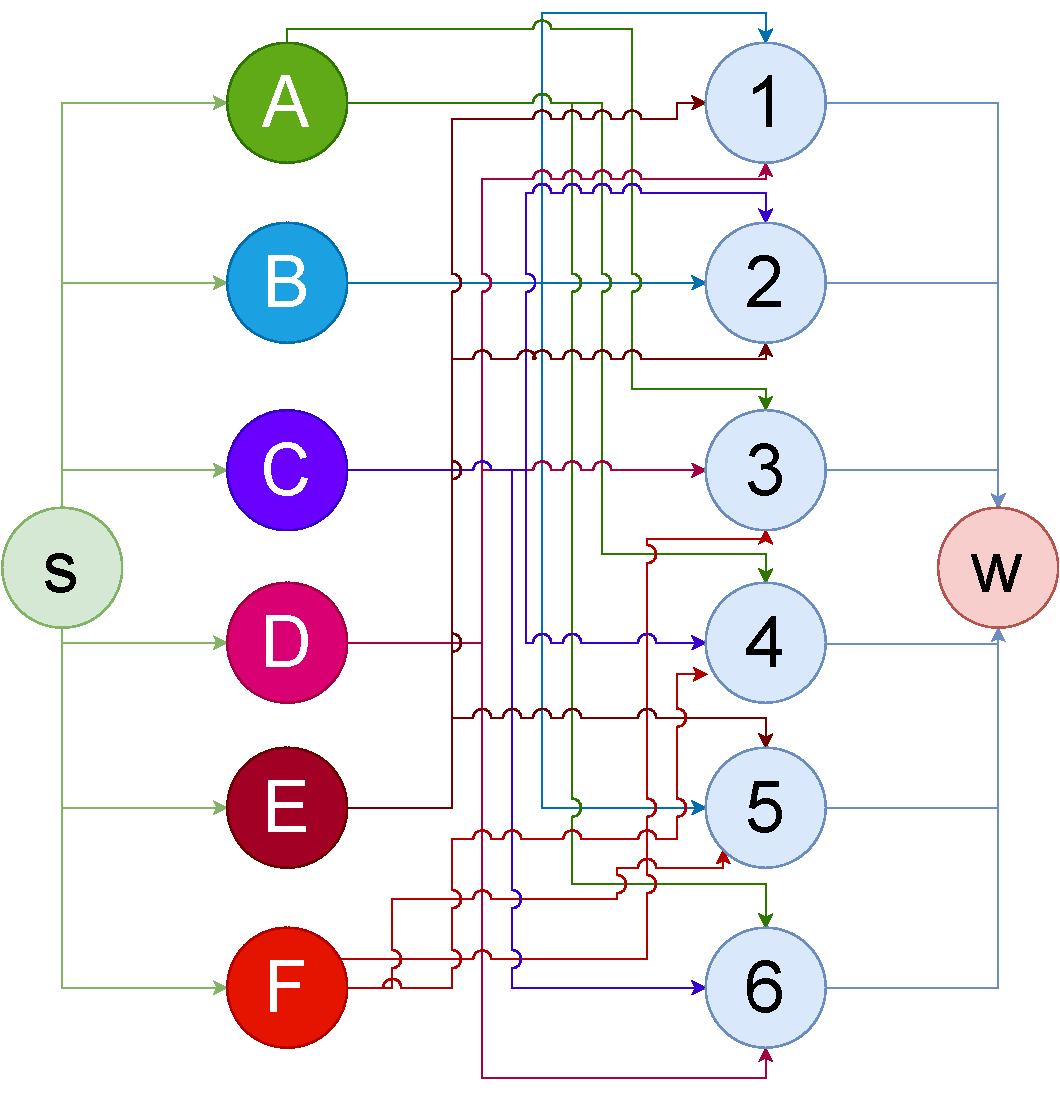
\includepdf[pages=-]{flowchart21.pdf}
\paragraph{Rozwiazanie}
\begin{lstlisting}[caption= plik dat]
data; 
 
set Wyjscie := t; 
set Wezly := 1, 2, 3, 4, 5, 6, A, B, C, D, E, F; 
set StartWezly := s, 1, 2, 3, 4, 5, 6, A, B, C, D, E, F; 
set WyjscieWezly := t, 1, 2, 3, 4, 5, 6, A, B, C, D, E, F; 
set StartWyjscieWezly := s, t, 1, 2, 3, 4, 5, 6, A, B, C, D, E, F; 
set Projekty := 1, 2, 3, 4, 5, 6; 
set Zespoly := A, B, C, D, E, F; 
 
param u := 
A 1 0 A 2 0 A 3 1 A 4 1 A 5 0 A 6 1
B 1 1 B 2 1 B 3 0 B 4 0 B 5 1 B 6 0 
C 1 1 C 2 0 C 3 1 C 4 0 C 5 0 C 6 1 
D 1 1 D 2 0 D 3 1 D 4 0 D 5 0 D 6 1 
E 1 1 E 2 1 E 3 0 E 4 0 E 5 1 E 6 0 
F 1 0 F 2 0 F 3 1 F 4 1 F 5 1 F 6 0; 
 
end; 
\end{lstlisting}
\begin{lstlisting}[caption= plik mod]
set Wyjscie; 
set Wezly; 
set StartWezly; 
set WyjscieWezly; 
set StartWyjscieWezly; 
set Projekty; 
set Zespoly; 
 
param u{z in Zespoly, p in Projekty}; 
 
var f{i in StartWyjscieWezly, j in StartWyjscieWezly}, >= 0; 
 
maximize Q: sum {p in Projekty, t in Wyjscie} f[p,t]; 
 
  Ograniczeni_jeden{i in StartWyjscieWezly, j in StartWyjscieWezly}: 
    f[i,j] >= 0; 
  Ograniczeni_dwa{i in StartWyjscieWezly, j in StartWyjscieWezly}: 
    f[i,j] <= 1; 
  Ograniczeni_trzy{p in Projekty, z in Zespoly}: 
    f[z,p] <= u[z,p]; 
  Ograniczeni_cztery{p in Projekty}: 
    sum {z in Zespoly} f[z,p] = 1; 
  Ograniczeni_piec{z in Zespoly}: 
    sum {p in Projekty} f[z,p] = 1; 
  Ograniczeni_szesc{n in Wezly}: 
    sum {i in WyjscieWezly} f[n,i] = sum {j in StartWezly} f[j,n]; 
	solve; 
display {i in Wezly, j in Wezly: f[i,j] > 0}: f[i,j]; 
display: Q;


\end{lstlisting}
\paragraph{Przydział zespołów do projektów}
\begin{lstlisting}[caption=wynik z glpk]
f[A,6].val = 1
f[B,5].val = 1
f[C,1].val = 1
f[D,3].val = 1
f[E,2].val = 1
f[F,4].val = 1
Q.val = 6
\end{lstlisting}
Wyniki: \\
Projekt numer \textbf{1} zostanie przydzielony zespołowi \textbf{C} \\
Projekt numer \textbf{2} zostanie przydzielony zespołowi \textbf{E} \\
Projekt numer \textbf{3} zostanie przydzielony zespołowi \textbf{D} \\
Projekt numer \textbf{4} zostanie przydzielony zespołowi \textbf{F} \\
Projekt numer \textbf{5} zostanie przydzielony zespołowi \textbf{B} \\
Projekt numer \textbf{6} zostanie przydzielony zespołowi \textbf{A} \\
\subsection{Zadanie 2.2 Minimalizacja kosztów realizacji projektów}
\paragraph{Problem do rozwiązania}
\begin{figure}[htb]
\caption{Koszty wynajmu}
\begin{center}
\begin{tabular}{ | c | c | c | c | c | c | c | }
\hline
  & A & B & C & D & E & F \\ 
 \hline
 1 & - & 13 & - & 14 & 18 & - \\  
 \hline
 2 & - & 4 & 2 & - & 3 & - \\
 \hline  
 3 & 2 & - & - & 10 & - & 13 \\
 \hline  
 4 & 10 & - & 5 & - & - & 15 \\
 \hline  
 5 & - & 10 & - & - & 17 & 12 \\
 \hline  
 6 & 20 & - & 6 & 16 & - & - \\
 \hline
\end{tabular}
\end{center}
\end{figure}

\begin{enumerate}
\item Parametry \\
s - źródło \\
w - wyjście \\
N - węzły (N = {s, t, 1, 2, 3, 4, 5, 6, A, B, C, D, E, F})
P - projekty (P = {1, 2, 3, 4, 5, 6} $\subseteq$ N)
Z - zespoły (Z = {A, B, C, D, E, F} $\subseteq$ N)
$k_{zp}$  - koszty przyporządkowania zespołu z do projektu p

\item Zmienne decyzyjne:
$f_{ij}$ - przeływ pomiędzy węzłem i oraz węzłem j
\item Funkcja celu
\begin{align*}
    Q &= \min \left(\sum_{z \in Z, p \in P} c_{zp}f_{zp} \right) \\
    &= \min \big( 13f_{B1} + 14f_{D1} + 18f_{E1} + 4f_{B2} + 2f_{C2} + 3f_{E2} \\
    &\quad + 2f_{A3} + 10f_{D3} + 13f_{F3} + 10f_{A4} + 5f_{C4} + 15f_{F4} \\
    &\quad + 10f_{B5} + 17f_{E5} + 12f_{F5} + 20f_{A6} + 6f_{C6} + 16f_{D6} \big)
\end{align*}


\item Ograniczenia
\setcounter{equation}{0}
\begin{equation}
0 \leq f_{ij} \leq 1, (i, j) \in N
\end{equation}
\begin{equation}
f_{si} = 0, i \in \{ s, t, 1, 2, 3, 4, 5, 6 \}
\end{equation}
\begin{equation}
f_{is} = 0, i \in N
\end{equation}
\begin{equation}
f_{ti} = 0, i \in N
\end{equation}
\begin{equation}
f_{it} = 0, i \in \{s, t, A, B, C, D, E, F\}
\end{equation}
\begin{equation}
\sum_{z \in Z} f_{zp} = 1, p \in P = \{ 1, 2, 3, 4, 5, 6 \}
\end{equation}
\begin{equation}
\sum_{p \in P} f_{zp} = 1, z \in Z = \{ A, B, C, D, E, F \}
\end{equation}
\begin{equation}
\sum_{i \in N \backslash \{s\}} f_{ni} = \sum_{j \in N \backslash \{t\}} f_{jn}, n \in N \backslash \{ s, t \}
\end{equation}

\end{enumerate}
\paragraph{Model sieciowy rysunek}
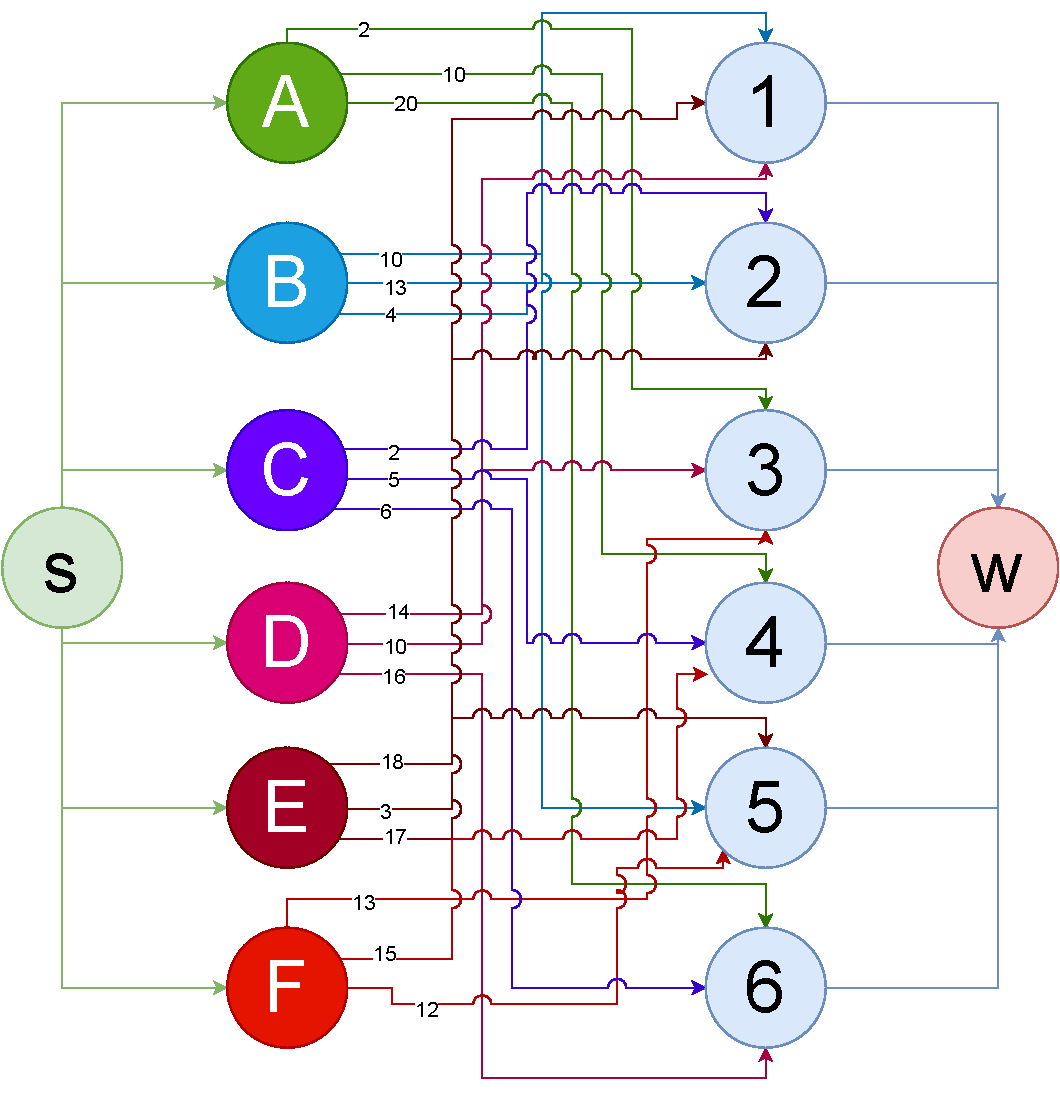
\includepdf[pages=-]{flowchart22.pdf}
\paragraph{Rozwiazanie}
\begin{lstlisting}[caption= plik dat]
data; 
 
set Wyjscie := t; 
set Wezly := 1, 2, 3, 4, 5, 6, A, B, C, D, E, F; 
set StartWezly := s, 1, 2, 3, 4, 5, 6, A, B, C, D, E, F; 
set WyjscieWezly := t, 1, 2, 3, 4, 5, 6, A, B, C, D, E, F; 
set StartWyjscieWezly := s, t, 1, 2, 3, 4, 5, 6, A, B, C, D, E, F; 
set Projekty := 1, 2, 3, 4, 5, 6; 
set Zespoly := A, B, C, D, E, F; 
 
param k := 
A 1 1000 A 2 1000 A 3 2 A 4 10 A 5 1000 A 6 20
B 1 13 B 2 4 B 3 1000 B 4 1000 B 5 10 B 6 1000 
C 1 1000 C 2 2 C 3 1000 C 4 5 C 5 1000 C 6 6 
D 1 14 D 2 1000 D 3 10 D 4 1000 D 5 1000 D 6 16 
E 1 18 E 2 3 E 3 1000 E 4 1000 E 5 17 E 6 1000 
F 1 1000 F 2 1000 F 3 13 F 4 15 F 5 12 F 6 1000; 
 
end; 
\end{lstlisting}
\begin{lstlisting}[caption= plik mod]
set Wyjscie; 
set Wezly; 
set StartWezly; 
set WyjscieWezly; 
set StartWyjscieWezly; 
set Projekty; 
set Zespoly; 
 
param k{z in Zespoly, p in Projekty}; 
 
var f{i in StartWyjscieWezly, j in StartWyjscieWezly}, >= 0; 
 
minimize Q: sum {p in Projekty, z in Zespoly} k[z, p] * f[z, p]; 
 
  Ograniczenie_jeden{i in StartWyjscieWezly, j in StartWyjscieWezly}: 
    f[i,j] >= 0; 
  Ograniczenie_dwa{i in StartWyjscieWezly, j in StartWyjscieWezly}: 
    f[i,j] <= 1; 
  Ograniczenie_trzy{p in Projekty}: 
    sum {z in Zespoly} f[z,p] = 1; 
  Ograniczenie_cztery{z in Zespoly}: 
    sum {p in Projekty} f[z,p] = 1; 
  Ograniczenie_piec{n in Wezly}: 
    sum {i in WyjscieWezly} f[n,i] = sum {j in StartWezly} f[j,n]; 
	solve; 
display {i in Wezly, j in Wezly: f[i,j] > 0}: f[i,j]; 
display: Q;



\end{lstlisting}
\paragraph{Przydział zespołów do projektów}
\begin{lstlisting}[caption=wynik z glpk]
f[A,3].val = 1
f[B,5].val = 1
f[C,6].val = 1
f[D,1].val = 1
f[E,2].val = 1
f[F,4].val = 1
Q.val = 50
\end{lstlisting}
Wyniki: \\
Projekt numer \textbf{1} zostanie przydzielony zespołowi \textbf{D} \\
Projekt numer \textbf{2} zostanie przydzielony zespołowi \textbf{E} \\
Projekt numer \textbf{3} zostanie przydzielony zespołowi \textbf{A} \\
Projekt numer \textbf{4} zostanie przydzielony zespołowi \textbf{F} \\
Projekt numer \textbf{5} zostanie przydzielony zespołowi \textbf{B} \\
Projekt numer \textbf{6} zostanie przydzielony zespołowi \textbf{C} \\
\subsection{Zadanie 2.3 Minimalizacja terminu realizacji puli projektów}
\begin{figure}[htb]
\caption{Czas realizacji projektów}
\begin{center}
\begin{tabular}{ | c | c | c | c | c | c | c | }
\hline
  & A & B & C & D & E & F \\ 
 \hline
 1 & - & 13 & - & 14 & 18 & - \\  
 \hline
 2 & - & 4 & 2 & - & 3 & - \\
 \hline  
 3 & 2 & - & - & 10 & - & 13 \\
 \hline  
 4 & 10 & - & 5 & - & - & 15 \\
 \hline  
 5 & - & 10 & - & - & 17 & 12 \\
 \hline  
 6 & 20 & - & 6 & 16 & - & - \\
 \hline
\end{tabular}
\end{center}
\end{figure}

\begin{enumerate}
\item Parametry \\
s - źródło \\
w - wyjście \\
N - węzły (N = {s, t, 1, 2, 3, 4, 5, 6, A, B, C, D, E, F})
P - projekty (P = {1, 2, 3, 4, 5, 6} $\subseteq$ N)
Z - zespoły (Z = {A, B, C, D, E, F} $\subseteq$ N)
$t_{zp}$  - czas realizacji projektu p przez zespół z [w miesiącach]

\item Zmienne decyzyjne:
$f_{ij}$ - przeływ pomiędzy węzłem i oraz węzłem j
\item Funkcja celu
\begin{align*}
    Q &= \min \left( \max_{z \in Z, p \in P} c_{zp} f_{zp} \right) \\
    &= \min \big\{13f_{B1}, 14f_{D1}, 18f_{E1}, 4f_{B2}, 2f_{C2}, 3f_{E2}, \\
    &\quad  2f_{A3}, 10f_{D3},13f_{F3}, 10f_{A4}, 5f_{C4}, 15f_{F4} \\
    &\quad 10f_{B5}, 17f_{E5}, 12f_{F5}, 20f_{A6}, 6f_{C6}, 16f_{D6} \big\}
\end{align*}


\item Ograniczenia
\setcounter{equation}{0}
\begin{equation}
0 \leq f_{ij} \leq 1, \; (i, j) \in N
\end{equation}
\begin{equation}
f_{si} = 0, \; i \in \{ s, t, 1, 2, 3, 4, 5, 6 \}
\end{equation}
\begin{equation}
f_{is} = 0, \; i \in N
\end{equation}
\begin{equation}
f_{ti} = 0, \; i \in N
\end{equation}
\begin{equation}
f_{it} = 0, \; i \in \{s, t, A, B, C, D, E, F\}
\end{equation}
\begin{equation}
\sum_{z \in Z} f_{zp} = 1, \; p \in P = \{ 1, 2, 3, 4, 5, 6 \}
\end{equation} 
\begin{equation}
\sum_{p \in P} f_{zp} = 1, \; z \in Z = \{ A, B, C, D, E, F \}
\end{equation}
\begin{equation}
\sum_{i \in N \backslash \{s\}} f_{ni} = \sum_{j \in N \backslash \{t\}} f_{jn}, \; n \in N \backslash \{ s, t \}
\end{equation}

\end{enumerate}
\paragraph{Model sieciowy rysunek}
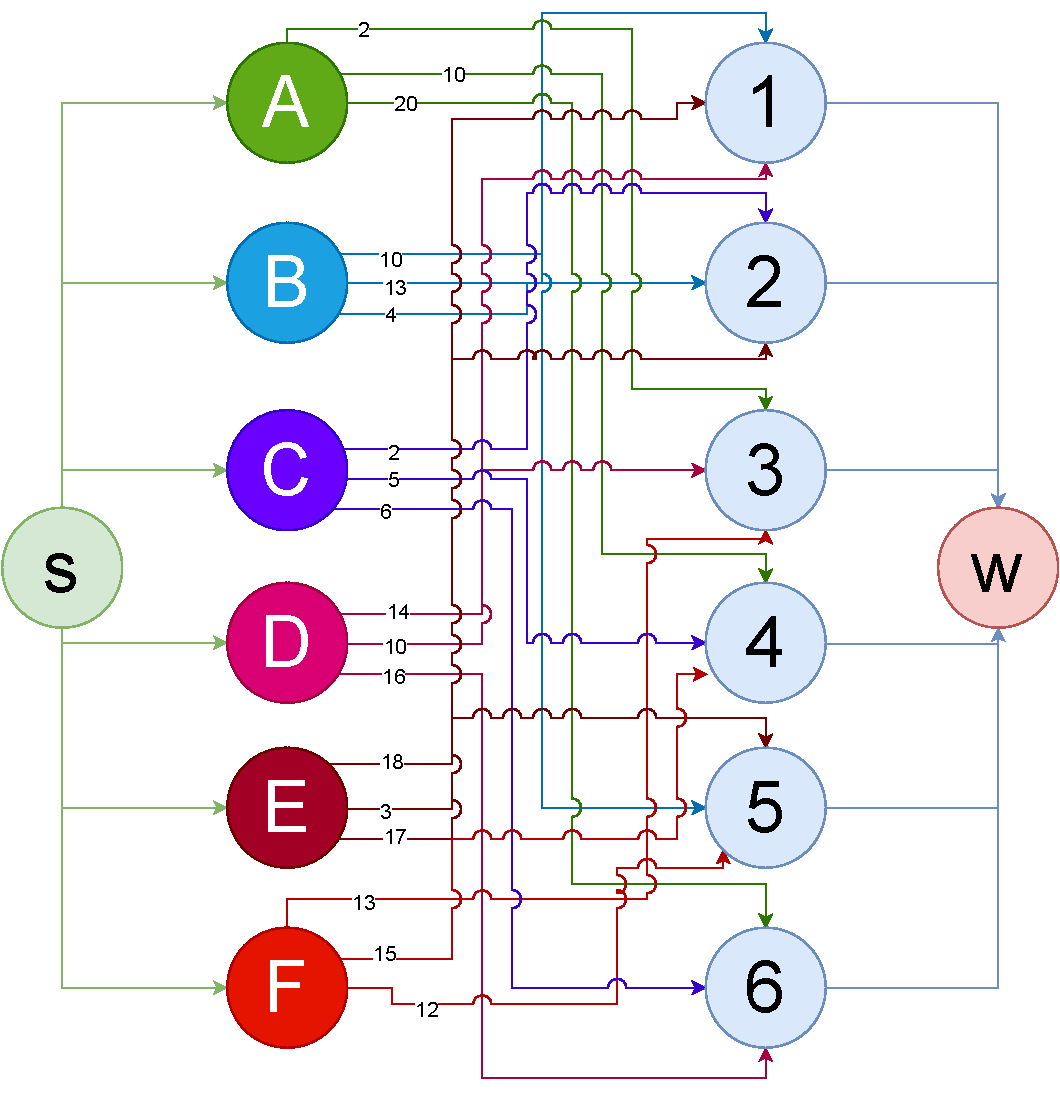
\includepdf[pages=-]{flowchart22.pdf}
\paragraph{Model programowania liniowego}
\begin{lstlisting}[caption= plik dat]
data; 
 
set Wyjscie := t; 
set Wezly := 1, 2, 3, 4, 5, 6, A, B, C, D, E, F; 
set StartWezly := s, 1, 2, 3, 4, 5, 6, A, B, C, D, E, F; 
set WyjscieWezly := t, 1, 2, 3, 4, 5, 6, A, B, C, D, E, F; 
set StartWyjscieWezly := s, t, 1, 2, 3, 4, 5, 6, A, B, C, D, E, F; 
set Projekty := 1, 2, 3, 4, 5, 6; 
set Zespoly := A, B, C, D, E, F; 
 
param c := 
A 1 1000 A 2 1000 A 3 2 A 4 10 A 5 1000 A 6 20
B 1 13 B 2 4 B 3 1000 B 4 1000 B 5 10 B 6 1000 
C 1 1000 C 2 2 C 3 1000 C 4 5 C 5 1000 C 6 6 
D 1 14 D 2 1000 D 3 10 D 4 1000 D 5 1000 D 6 16 
E 1 18 E 2 3 E 3 1000 E 4 1000 E 5 17 E 6 1000 
F 1 1000 F 2 1000 F 3 13 F 4 15 F 5 12 F 6 1000; 
 
end; 
\end{lstlisting}
\begin{lstlisting}[caption= plik mod]
set Wyjscie; 
set Wezly; 
set StartWezly; 
set WyjscieWezly; 
set StartWyjscieWezly; 
set Projekty; 
set Zespoly; 
 
param c{z in Zespoly, p in Projekty}; 
 
var f{i in StartWyjscieWezly, j in StartWyjscieWezly}, >= 0, integer; 
var cmax, >= 0; 
 
minimize Q: cmax; 
 
subject to
  Ograniczenie_jeden{i in StartWyjscieWezly, j in StartWyjscieWezly}: 
    f[i,j] >= 0; 
  Ograniczenie_dwa{i in StartWyjscieWezly, j in StartWyjscieWezly}: 
    f[i,j] <= 1; 
  Ograniczenie_trzy{p in Projekty}: 
    sum {z in Zespoly} f[z,p] = 1; 
  Ograniczenie_cztery{z in Zespoly}: 
    sum {p in Projekty} f[z,p] = 1; 
  Ograniczenie_piec{n in Wezly}: 
    sum {i in WyjscieWezly} f[n,i] = sum {j in StartWezly} f[j,n]; 
	Ograniczenie_szesc{z in Zespoly, p in Projekty}: 
		c[z,p] * f[z,p] <= cmax;
solve;
display {i in Wezly, j in Wezly: f[i,j] > 0}: f[i,j]; 
display: Q;
\end{lstlisting}

\begin{lstlisting}[caption=wynik z glpk]
f[A,4].val = 1
f[B,1].val = 1
f[C,6].val = 1
f[D,3].val = 1
f[E,2].val = 1
f[F,5].val = 1
Q.val = 13
\end{lstlisting}
Wyniki: \\
Projekt numer \textbf{1} zostanie przydzielony zespołowi \textbf{B} \\
Projekt numer \textbf{2} zostanie przydzielony zespołowi \textbf{E} \\
Projekt numer \textbf{3} zostanie przydzielony zespołowi \textbf{D} \\
Projekt numer \textbf{4} zostanie przydzielony zespołowi \textbf{A} \\
Projekt numer \textbf{5} zostanie przydzielony zespołowi \textbf{F} \\
Projekt numer \textbf{6} zostanie przydzielony zespołowi \textbf{C} \\
\section{Zadanie 3}
\paragraph{Model programowania liniowego}
\begin{enumerate}
\item Parametry \\
m - liczba różnych zasobów, i $\in$ N \\ 
n - liczba różnych produktów, j $\in$ N \\
$c_{i}^{max}$ - Maksymalna przepustowość dla zasobu i \\
$A_{ij}$ - Użycie zasobu i przez produkt j \\ 
$q_j$ - Limit produkcji dla produktu j, po którym zmniejsza się przychód na jednostce \\
$p_j$ - Normalny przychód na pojedyńczej sztuce produktu j \\ 
$p_j^{disc}$ - Pomniejszony przychód na sztuce produktu j 

\item Zmienne decyzyjne 
$x_j$ - Wolumin produkcji produktu j 
\item Zmienne pomocnicze 
$r_j(u)$ - Funkcja wyliczająca przychód dla produktu j bazując na poziomie produkcji u \\ 
$c_i$ - Całkowite zużycie zasobu typu i 

\item Funkcja celu 
\[ \max Z = \sum_{j=1}^n r_j u_j \] 
\[ r_j(u) = \{ \]
\[    p_{j} u \qquad \qquad \qquad \qquad u <= q_j  \]
\[    p_j q_j + p_{j}^{disc}(u-q_j), \qquad u => q_j \]
\[ \} \]

\item Ograniczenia 
\setcounter{equation}{0}
Całkowite zużycie zasobów nie może przekraczać dostępnośli dla żadnego zasobu
\begin{equation}
\sum_{j=1}^n A_{ij} \cdot x_j \leq c_i^{max}, \qquad i \in N
\end{equation}
Produkcja każdego produktu j, jest powiżana z właściwym $u_j$
\begin{equation}
u_j = x_j, \qquad j \in N
\end{equation}
Wolumin produkcji nie może być mniejszy od zera
\begin{equation}
x_j \geq 0, \qquad j \in N
\end{equation}


\end{enumerate}
\end{document}

